% Copyright (c) 2026 Islam Ibrahim. All rights reserved.

\documentclass[tikz,border=10pt]{standalone}
\usepackage[T1]{fontenc}
\usepackage{lmodern}
\usepackage{amsmath}
\usepackage{tikz}
\usetikzlibrary{positioning}

\begin{document}

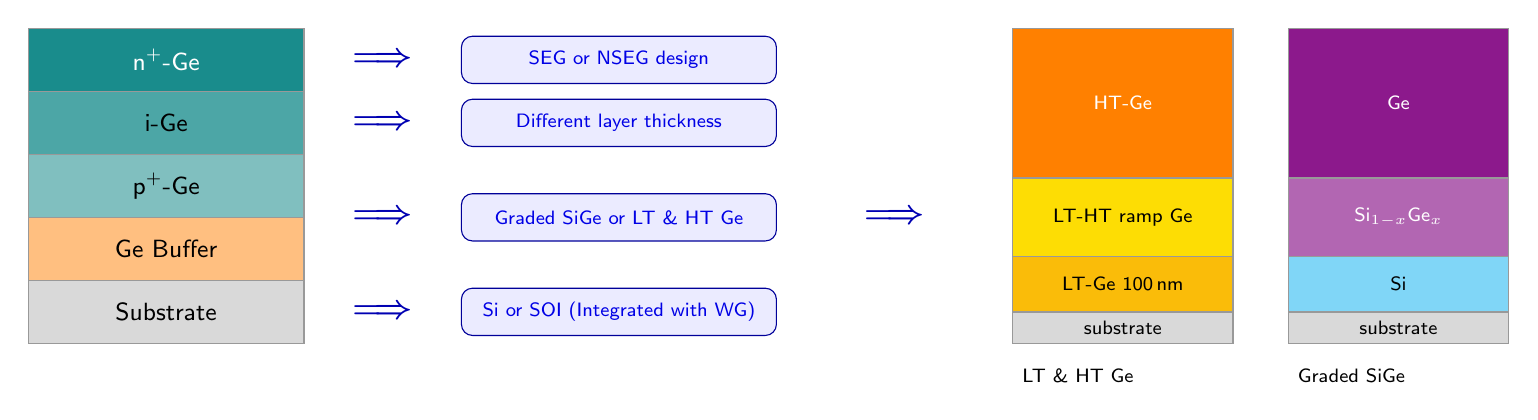
\begin{tikzpicture}[font=\small\rmfamily]

% ---- Define Styles ----
\tikzset{
  mainlayer/.style={
    draw=gray!80, line width=0.5pt, minimum width=3.5cm, minimum height=0.8cm, 
    font=\small\sffamily, align=center, outer sep=0pt, anchor=south west
  },
  rightlayer/.style={
    draw=gray!80, line width=0.5pt, minimum width=2.8cm,
    font=\scriptsize\sffamily, align=center, outer sep=0pt, anchor=south west
  },
  optionbox/.style={
    draw=blue!60!black, fill=blue!8, rounded corners=4pt,
    minimum width=4.0cm, minimum height=0.6cm,
    font=\scriptsize\sffamily, align=center, text=blue!90!black, anchor=center
  }
}

% Custom robust block arrow (Bold mathLongrightarrow)
\newcommand{\blockarrow}{$\boldsymbol{\Longrightarrow}$}

% =========================================================
% LEFT STACK (Main Device)
% Total height = 4.0 cm (5 layers of 0.8 cm each)
% =========================================================
\node[mainlayer, fill=gray!30]             (sub) at (0, 0.0) {Substrate};
\node[mainlayer, fill=orange!50]           (buf) at (0, 0.8) {Ge Buffer};
\node[mainlayer, fill=teal!50]             (pge) at (0, 1.6) {p$^+$-Ge};
\node[mainlayer, fill=teal!70]             (ige) at (0, 2.4) {i-Ge};
\node[mainlayer, fill=teal!90, text=white] (nge) at (0, 3.2) {n$^+$-Ge};

% =========================================================
% MIDDLE OPTION BOXES
% Centers aligned exactly with left stack layers/boundaries
% =========================================================
\node[optionbox] (opt1) at (7.5, 3.6) {SEG or NSEG design};
\node[optionbox] (opt2) at (7.5, 2.8) {Different layer thickness};
% Y=1.6 is exactly centered between Ge Buffer (0.8-1.6) and p+-Ge (1.6-2.4)
\node[optionbox] (opt3) at (7.5, 1.6) {Graded SiGe or LT \& HT Ge};
\node[optionbox] (opt4) at (7.5, 0.4) {Si or SOI (Integrated with WG)};

% =========================================================
% BLOCK ARROWS: Left Stack -> Options
% =========================================================
% Y-centers match exactly for perfect horizontal alignment
\node[font=\large, text=blue!70!black] at (4.5, 3.6) {\blockarrow};
\node[font=\large, text=blue!70!black] at (4.5, 2.8) {\blockarrow};
\node[font=\large, text=blue!70!black] at (4.5, 1.6) {\blockarrow}; % Originates at the boundary
\node[font=\large, text=blue!70!black] at (4.5, 0.4) {\blockarrow};

% =========================================================
% RIGHT STACK 1: LT & HT Ge
% Total height = 4.0 cm (0.4 + 0.7 + 1.0 + 1.9)
% Designed so ramp center is exactly at Y=1.6
% =========================================================
\def\rx{12.5}
\node[rightlayer, fill=gray!30, minimum height=0.4cm] (lsub) at (\rx, 0.0) {substrate};
\node[rightlayer, fill=yellow!50!orange, minimum height=0.7cm] (ltge) at (\rx, 0.4) {LT-Ge 100\,nm};
\node[rightlayer, fill=yellow!80!orange, minimum height=1.0cm] (ramp) at (\rx, 1.1) {LT-HT ramp Ge};
\node[rightlayer, fill=red!50!yellow, text=white, minimum height=1.9cm] (htge) at (\rx, 2.1) {HT-Ge};

\node[below=0.2cm of lsub.south west, anchor=north west, font=\scriptsize\sffamily] (lblA) {LT \& HT Ge};

% =========================================================
% RIGHT STACK 2: Graded SiGe
% Total height = 4.0 cm (0.4 + 0.7 + 1.0 + 1.9)
% Designed so SiGe center is exactly at Y=1.6
% =========================================================
\def\rxx{16.0}
\node[rightlayer, fill=gray!30, minimum height=0.4cm] (gsub) at (\rxx, 0.0) {substrate};
\node[rightlayer, fill=cyan!50, minimum height=0.7cm] (si) at (\rxx, 0.4) {Si};
\node[rightlayer, fill=violet!60, text=white, minimum height=1.0cm] (sige) at (\rxx, 1.1) {Si$_{1-x}$Ge$_x$};
\node[rightlayer, fill=violet!90, text=white, minimum height=1.9cm] (ge) at (\rxx, 2.1) {Ge};

\node[below=0.2cm of gsub.south west, anchor=north west, font=\scriptsize\sffamily] (lblB) {Graded SiGe};

% =========================================================
% BLOCK ARROW: Options -> Right Stack
% Direct single arrow to LT-HT ramp Ge
% =========================================================
% Positioned perfectly halfway between the option box (ends at 9.5) and ramp (starts at 12.5)
\node[font=\large, text=blue!70!black] at (11.0, 1.6) {\blockarrow};

\end{tikzpicture}

\end{document}